\section{Tool requirements}
    \label{sec:requirements} 

    The goal to be achieved is to integrate project manager, requirements engineers, and product designers with the corresponding CAD data to create a compact and lightweight tool to support product development. Customers and companies can evaluate and control the development status on a common basis. For this purpose, the platform GitHub was considered as a reference, which already offers a similar solution in the area of software development. The tool we are developing should be able to run platform independently on different devices. To involve the customer in the development process clear user roles with corresponding permissions must be defined. Each added version of a product contains a new CAD model with version number, base version and description. For each product it should be possible to create issues, which are filtered by open and closed issues. 
    In each issue there should be a communication channel in which the issues can be discussed. 
    Here, the user should be able to select and reference specific components to the text and open and close the corresponding issues. 
    Another level of product management is built by the milestones. Milestones can be created, and different issues can be added to them. A list of open and closed issues as well as a chart show the progress of each milestone. Finally, the platform must provide settings for each product to define the member list and the product properties. All data generated on the platform should be stored in a database.

\section{Tool design}
    \label{sec:contribution}

    In the following, we present our tool design consisting of four models: An integrated data model, a function model, a permission model, and an interface model.
    The integrated data model describes the representation of CAD model revisions, design tasks, and project schedules.
    The function model explains the change operations stakeholders can perform on top of the data model.
    The permission model outlines which functions can be used by which stakeholder depending on his/her role.
    Finally, an interface model demonstrates how the previous models can be put into action practically.

    \subsection*{Data model}

    \begin{figure*}[ht]
        \centering
        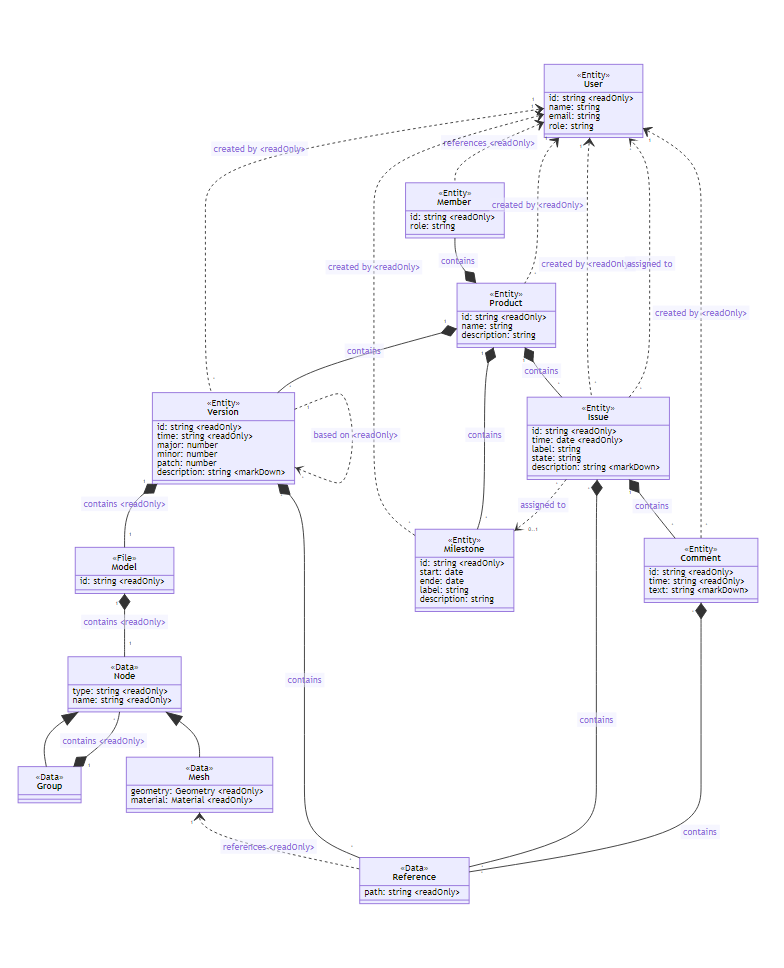
\includegraphics[width=\textwidth]{entities-v5.png}
        \caption{Data model}
        \label{fig: datamodel}
    \end{figure*}

    The core of the software is in the backend. Via the API, the data can be manipulated using CRUD methods. This section describes the data model of the software. The necessary classes and entities are based on the interfaces in the common package.
    The data model contains the following entities as shown in Figure~\ref{fig: datamodel}: \textit{User, Product, Version, Issue, Comment, Milestone, Member}. At the top level of the data model is the user, who can create multiple products if he has the permission to do so. For each product versions, issues, milestones and members can be created. The entity \textit{user} User has personal attributes like name, email, password and the two permissions to create and change users or to create products. Finally, like any other entity, the user has a \textit{deleted} flag. If the deletes an entity this is set to true. All other entities like \textit{Version, Issue, Comment, Milestone and Member} are linked to the product entity. The product itself does not provide much information, because the information is primarily in the linked entities. The versions of a product contain important information and the 3D CAD model in the format glTF\footnote{\url{https://www.khronos.org/gltf/}}. This data format can be rendered well in web applications and runs very performant in the browser.  To create a semantic versioning, the attributes major, minor and patch are specified for a version. By knowing the current version and previous version, a version history can be implemented. Multiple issues can be added for each product. The \textit{state} attribute distinguishes between \textit{open} and \textit{closed} issues. So it is possible to filter for completed and not completed issues. For each issue one or more comments can be created. With the attribute \textit{action} an issue can be closed or reopened by the comment. The text in a comment is compatible with markdown
    For each product one or more milestones can be defined. These have a label and start and end dates. For each product one or more members can be added. The attribute \textit{role} can have three states: \textit{manager, engineer, customer}. Depending on the role, the corresponding product member has different permissions to interact with the respective product  as defined in the persmission model in Section~\ref{subsec:permissionModel}. 

    \subsection*{Function model} 
    The functions implemented in the API allow to create, read, update, search and delete data to interact with the data model. This would not even require a graphical user interface. All functions offered by the API are called via HTTP requests. These requests can also be made via the console or other software such as Postman\footnote{https://www.postman.com/} or Swagger\footnote{https://swagger.io}. Thus, the functional model in combination with the data model is the foundation of this application. 
    By triggering a function in the API, various permission checks are executed to verify if the active user has the permission for performing this action as specified in the permission model in Section~\ref{subsec:permissionModel}. 

    \subsubsection*{User management}
    Users can be found, created, modified and deleted. Permissions can be assigned to allow the new user to create and edit other users and to create products. For this the two flags \textit{user management permission (ump)} and \textit{product management permission (pmp)} must be set. The API offers the following methods for interaction with user objects:
    \texttt{\begin{itemize} 
        \item addUser(email: string, name: string, passwort: string, ump: boolean, pmp: boolean, file?: File)
        \item updateUser(id: string, email: string, name: string, passwort: string, ump: boolean, pmp: boolean, file?: File)
        \item deleteUser(id: string)
        \item findUsers(query?: string, productId?: string) 
        \item getUser(id: string)
    \end{itemize}}

     For the \texttt{addUser} method the input parameter is needed, which contains the information about the new user. The second parameter holds the profile picture and is optional.  \texttt{UpdateUser} needs the user ID, the new data and optionally a file containing a profile picture. \texttt{DeleteUser} sets the \textit{deleted} flag of the particular user to true. 
     The \texttt{findUsers} method searches for all users of the system from the database. It can be searched either via a query by username or via the product ID. The parameters \textit{query} and \textit{productId} are optional.
     \texttt{GetUser} searches for a specific user based on the user ID and returns the object.
     The \texttt{GetUser} and \texttt{addUser} methods are implemented that way, to search for objects that are not deleted.

    \subsubsection*{Product management}
    This part of the API provides methods to interact with product objects. Here products can be created, modified, searched and deleted. The following list shows the methods that are available for interacting with products:
    \texttt{
        \begin{itemize}
            \item addProduct(userId: string, name: string, description: string)
            \item updateProduct(id: string, name: string, description: string)
            \item deleteProduct(id: string)
            \item findProducts()
            \item getProduct(id: string)
        \end{itemize}
    }

    The methods work according to the same principle as in user management. It is searched with the corresponding product ID for the object or its attributes get changed. When deleting a product, it must be ensured that all objects that are attached to a product are also deleted. So if a product is deleted, all versions, issues, milestones and members must also be deleted.
    The \texttt{findProducts} method searches in the database for all products that are not deleted. For this no passing parameter is necessary.
    
    \subsubsection*{Version management}
    Again, the API provides CRUD methods to interact with versions:
   \texttt{
        \begin{itemize}
            \item addVersion(userId: string, productId: string, baseVersionIds: string[], time: timestamp, major: number, minor: number, patch: number, description: string, file: File)
            \item updateVersion(id: string, major: number, minor: number, patch: number, description: string, file?: File)
            \item deleteVersion(id: string)
            \item findVersions(productId: string)
            \item getVersion(id: string)
        \end{itemize}
    }

    Unlike user management, a file must be specified when a version is created. 
    This CAD model can be exchanged when updating the version so that these can still be changed afterwards. The base versions cannot be changed later on.
    Since the versions are linked to a product, only the product ID can be used to search for it.

    \subsubsection*{Issue management} 
    These methods are available to create, read, find, update and delete issues:
    \texttt{ 
        \begin{itemize}
            \item addIssue(userId: string, productId: string, time: timestamp, label: string, text: string, state: 'open' or 'closed', assigneeIds: string[], milestoneId?: string)
            \item updateIssue(id: string, time: timestamp, label: string, text: string, state: 'open' or 'closed', assigneeIds: string[], milestoneId?: string)
            \item deleteIssue(id: string)
            \item findIssues(productId: string, milestoneId?: string, state?: 'open' or 'closed')
            \item getIssue(id: string)
        \end{itemize}
    }

    The \texttt{updateIssue} method is mainly used to update the list of assignees, change which milestones the issue belongs to and to close and reopen an issue.
    When deleting issues, all comments belonging to the respective issue must also be deleted.
    The \texttt{findIssues} method can search for issues in the database in several ways depending on the input parameters. Issues can be found by the product ID, the corresponding milestones or by the \textit{state} attribute to filter by open and closed issues.
    To filter by open and closed issues is especially useful to be able to filter for completed or uncompleted tasks for the purpose of product management. 
    
    \subsubsection*{Comment management}
    The following list shows the methods that can be performed to interact with the comment objects:
    \texttt{
        \begin{itemize}
            \item addComment(userId: string, issueId: string, time: timestamp, text: string, action: 'none' or 'close' or 'reopen')
            \item updateComment(id: string, text: string, action: 'none' or 'close' or 'reopen')
            \item deleteComment(id: string)
            \item findComments(issueId: string)
            \item getComment(id: string)
        \end{itemize}
    }

    The \texttt{addComment} method creates a comment with the given attributes. The user can define the action of the comment to interact with the corresponding issue. For example, if a comment is created with the action \textit{close}, the associated issue will be closed by triggering the \texttt{updateIssue} method which modifies the state of the issue. An issue can also be reopened in the same way by passing the according action. The action \textit{none} does not change the state of the issue. 
    With \texttt{updateComment} it is possible to modify the text or the action of an existing comment.
    The \texttt{deleteComment} method only deletes the corresponding Comment. Nothing else on the platform is deleted in the process. The actions of the comment remain until another comment performs another action. 

    \subsubsection*{Milestone management}
    Milestones are a container that can be filled with issues by reference. The CRUD methods are listed below:
    \texttt{
        \begin{itemize}
            \item addMilestone(userId: string, productId: string, label: string, start: timestamp, end: timestamp)
            \item updateMilestone(id: string, label: string, start: timestamp, end: timestamp)
            \item deleteMilestone(id: string)
            \item findMilestones(productId: string)
            \item getMilestone(id: string)
        \end{itemize}
    }

    The methods have analogous purposes as already with the other data objects. When deleting a milestone, it must be ensured that the references to the linked issues are removed.

    \subsubsection*{Member management}
    The API provides the following methods for member management:
    \texttt{
        \begin{itemize}
            \item addMember(productId: string, userId: string, role: 'manager' or 'engineer' or 'customer')
            \item updateMember(id: string, role: 'manager' or 'engineer' or 'customer')
            \item deleteMember(id: string)
            \item findMembers(productId: string, userId?: string)
            \item getMember(id: string)
        \end{itemize}
    }

    The \texttt{addMember} method creates new members for an existing product. With the input parameter \textit{role} different user roles can be distributed. If a combination of product and user already exists and is created a second time, they have different IDs compared to the original ones and are therefore independent. 
    The user ID can be used to find one specific member. Then the \texttt{findMembers} method returns an array of members. The other methods are similar to those of the other entities.

    \subsection*{Permission model}
    \label{subsec:permissionModel}
    The permission model offers a number of possible restrictions on the platform so that not every user has all freedoms. This is especially important when cooperating with customers. The customer should only have the possibility to evaluate existing products. For this he can see the products he is registered for and use the given product management functions depending on its member role \textit{customer}. Creating new users and products should only be possible by the managers of the respective product. They also organize the rights of each user. The permission model is divided into two levels. The first level is the global level and the second level is the product level. The global level uses a permission model and the product level a role model which is implicitly linked to the permission model. 
    This allows the first level to manage products and users and the role model to distribute more specific permissions to the individual products. This system is deeply integrated in the backend.

    \subsubsection*{Global level}
    The \textit{User} entity has the two attributes \textit{user management permission} and \textit{product management permission}. Only a user who has the user management permission can create or edit users. On the other hand every user can edit his own personal data. With the product management permission it is possible to create new products. If a new product is created, the respective user is automatically also a product member and receives the member role \textit{manager}. The permissions of each user can be adjusted afterwards. So it is possible to give multiple users the permissions for user management and product management. For example, a user and product manager can exist for each department. 

    \subsubsection*{Product level}
    For permission management at product level, three member roles are provided. These roles are: \textit{manager, engineer and customer}. The manager is the one who created the product and has the permission to add more members. So he can add more managers, who in turn have all the rights over the management of the product. This is useful when the product development covers several departments. The second role is the engineer. He is involved in the product development process. He has no rights to change the product description or its members. However, he can freely create and edit versions, issues and comments. The last role is the customer who has the possibility to observe the product development process. He can create issues and comments and so participate in the product development process. In the current version of the software the rights of the customer are still very strict. The permission system is implemented in such a way that it can be changed with few adjustments. If the customer needs writing permissions, this can be easily changed.
    
    \subsection*{Interface model} 
    The user interface provides a convenient way to interact with the functional model to display and modify data. The user interface offers a consistent design, which runs through the entire system.

    \subsubsection*{Product view}
    The \textit{product view} page lists all available products, for which the user has the permission to see them, in a table [see Fig. \ref{fig: startpage} on page~\pageref{fig: startpage}]. For each product in the table a preview is shown. The other columns show the attributes \textit{owner, name, description, versions, issues and members}. The X on the right provides the possibility to delete the corresponding product. The owner is the person who created the product. Name and description are defined when the product is created and can be changed later. The columns on the right show how many versions exist for this product, how many issues have been created and how many members have access to the product. By clicking on New product you get also to the ProductSettings view where you can add a new product when you have the product management permission. This button is only visible when the corresponding user has product management permission. The CAD model and version details will be added when the user creates a new version of a product.

    \begin{figure}[h]
        \centering
        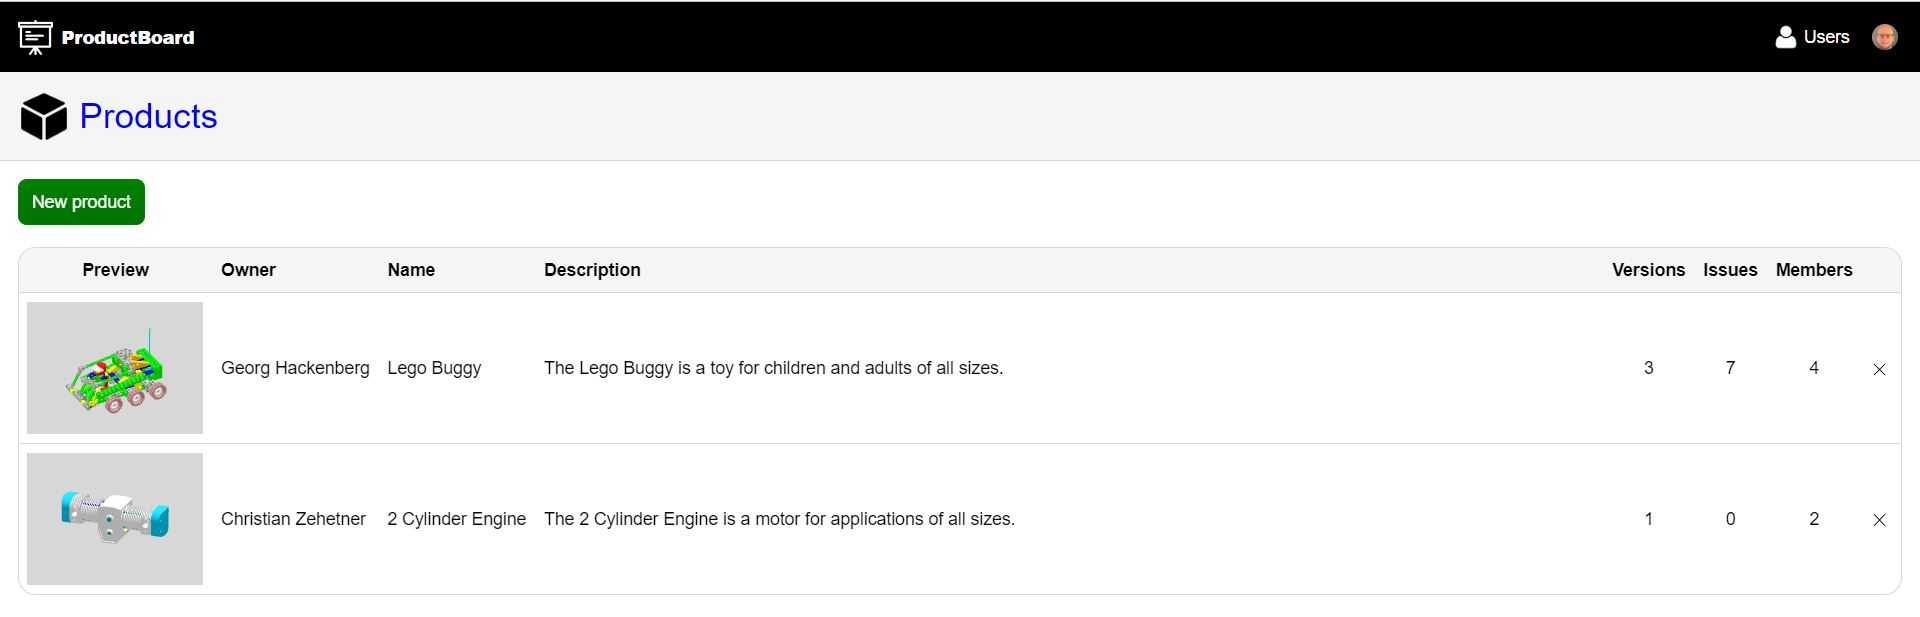
\includegraphics[width=\columnwidth]{startpage.JPG}
        \caption{Product view}
        \label{fig: startpage}
    \end{figure}

    \subsubsection*{ProductVersion view}
    Clicking on a product takes you to the ProductVersion view. You can also use the toolbar to jump to other pages such as issues, milestones members or settings. The left side of the view shows the created versions. On the left side there is a tree structure similar to GitHub. This tree structure results from the chronological arrangement of the product versions. The lines of the structure show how the product versions are in relation to the respective base versions. In the middle is the corresponding version number with the owner of the version inclusive email and a short description. Each version offers a preview. By clicking on the respective version, the 3D view on the right side also changes and shows the selected model. The 3D view allows to rotate, move and zoom the model. 
    With a click on the \textit{New version} button you get to the ProductVersionSettings view where you can create new product versions. [see Fig. \ref{fig: versionsettingsview} on page~\pageref{fig: versionsettingsview}]. 

    \subsubsection*{ProductVersionSettings view}
    Here you can enter information for a new version and select an GLB file. Depending on the selected base versions, the ProductVersion view shows the new version with the corresponding new tree structure after pressing the Save button. It is also possible to select multible base versions to merge them into a new version.

    \begin{figure}[h]
        \centering
        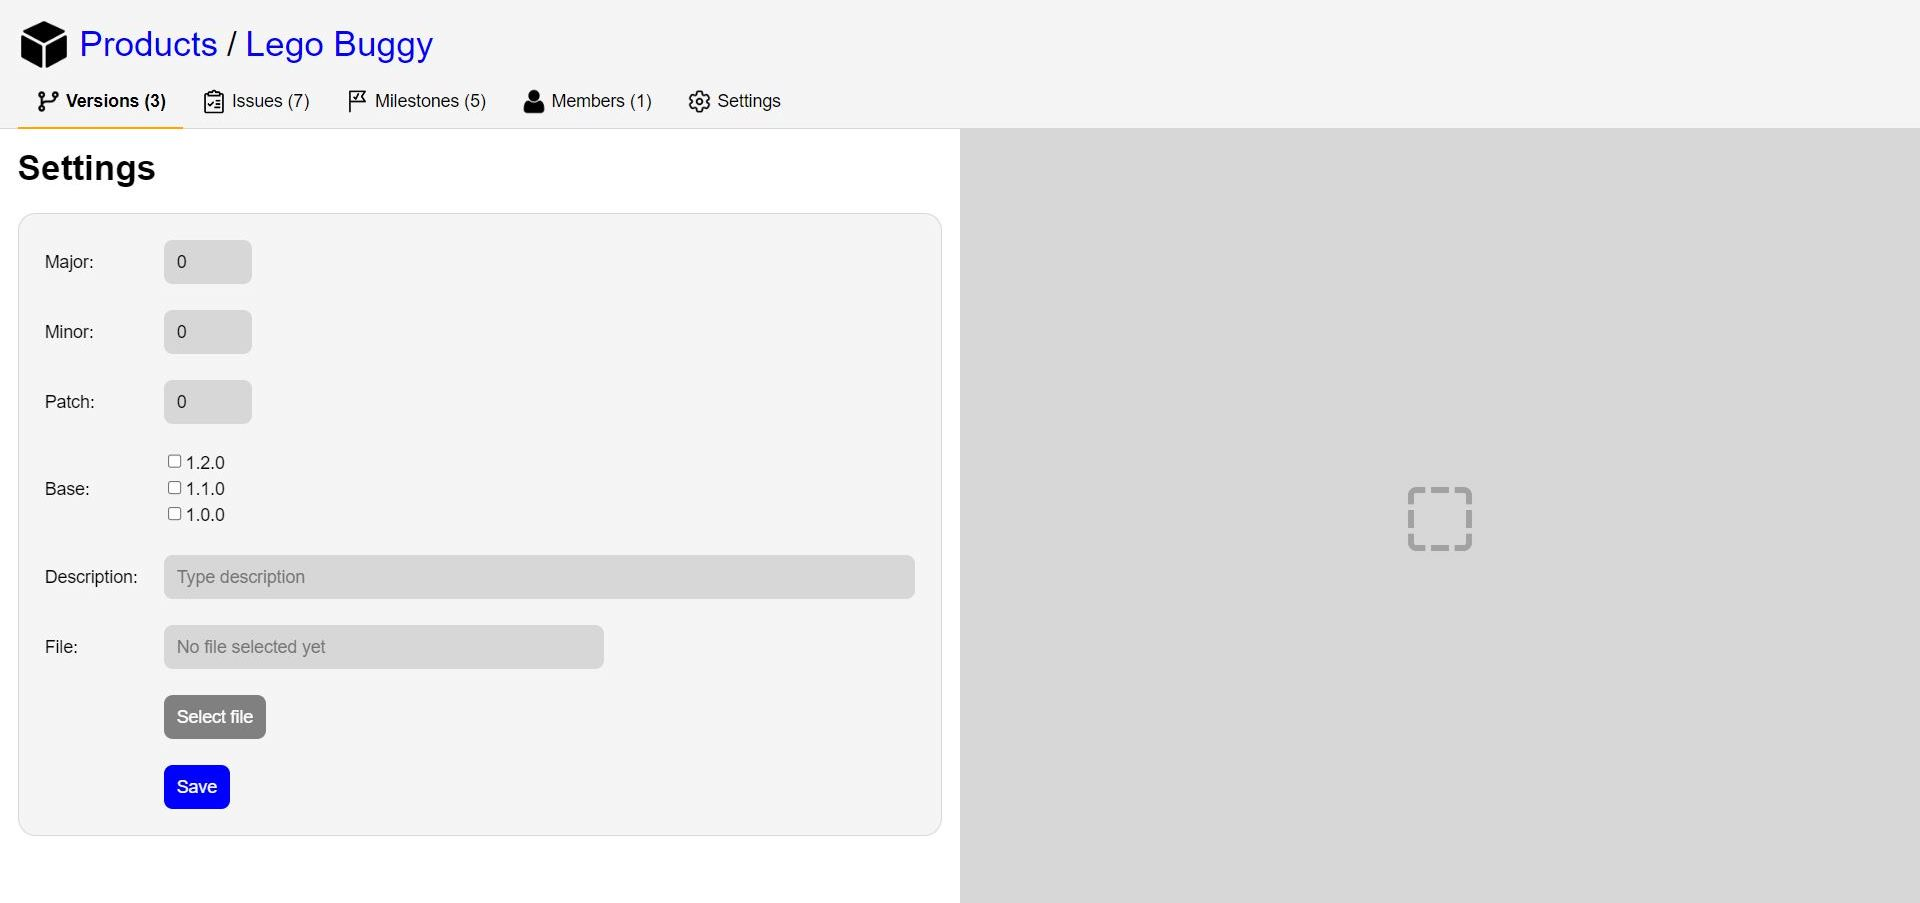
\includegraphics[width=\columnwidth]{versionsettingsview.JPG}
        \caption{ProductVersionSettings view}
        \label{fig: versionsettingsview}
    \end{figure}

    \subsubsection*{ProductIssue view}
    By clicking on the Issues link, you access the ProductIssue view [see Fig. \ref{fig: issueview} on page~\pageref{fig: issueview}]. Here the created issues are displayed in a table. The two buttons Open Issues and Closed Issues can be used to filter the list accordingly. The table shows the reporter who created the issue, the associated label, the assignees and how many comments and marked parts are in the conversation channel. 
    All views with 3D View offer the possibility to select a desired version for viewing. In the version view the version can be clicked directly. In the other views the version can be selected via a dropdown menu. This menu is located in the upper left corner of the 3D View. 
    If the user hovers with the mouse over a part of the 3D model, this part gets highlighted. 
    When hovering over an issue, the 3D view shows those parts that have been referenced in the comments of the respective issue by highlighting them in red.
    When hovering over an issue the parts are only highlighted if the version on which the parts were selected was picked in the dropdown menu. Thats because the 3d view shows for each version only the markers that were created on corresponding version.

    \begin{figure}[h]
        \centering
        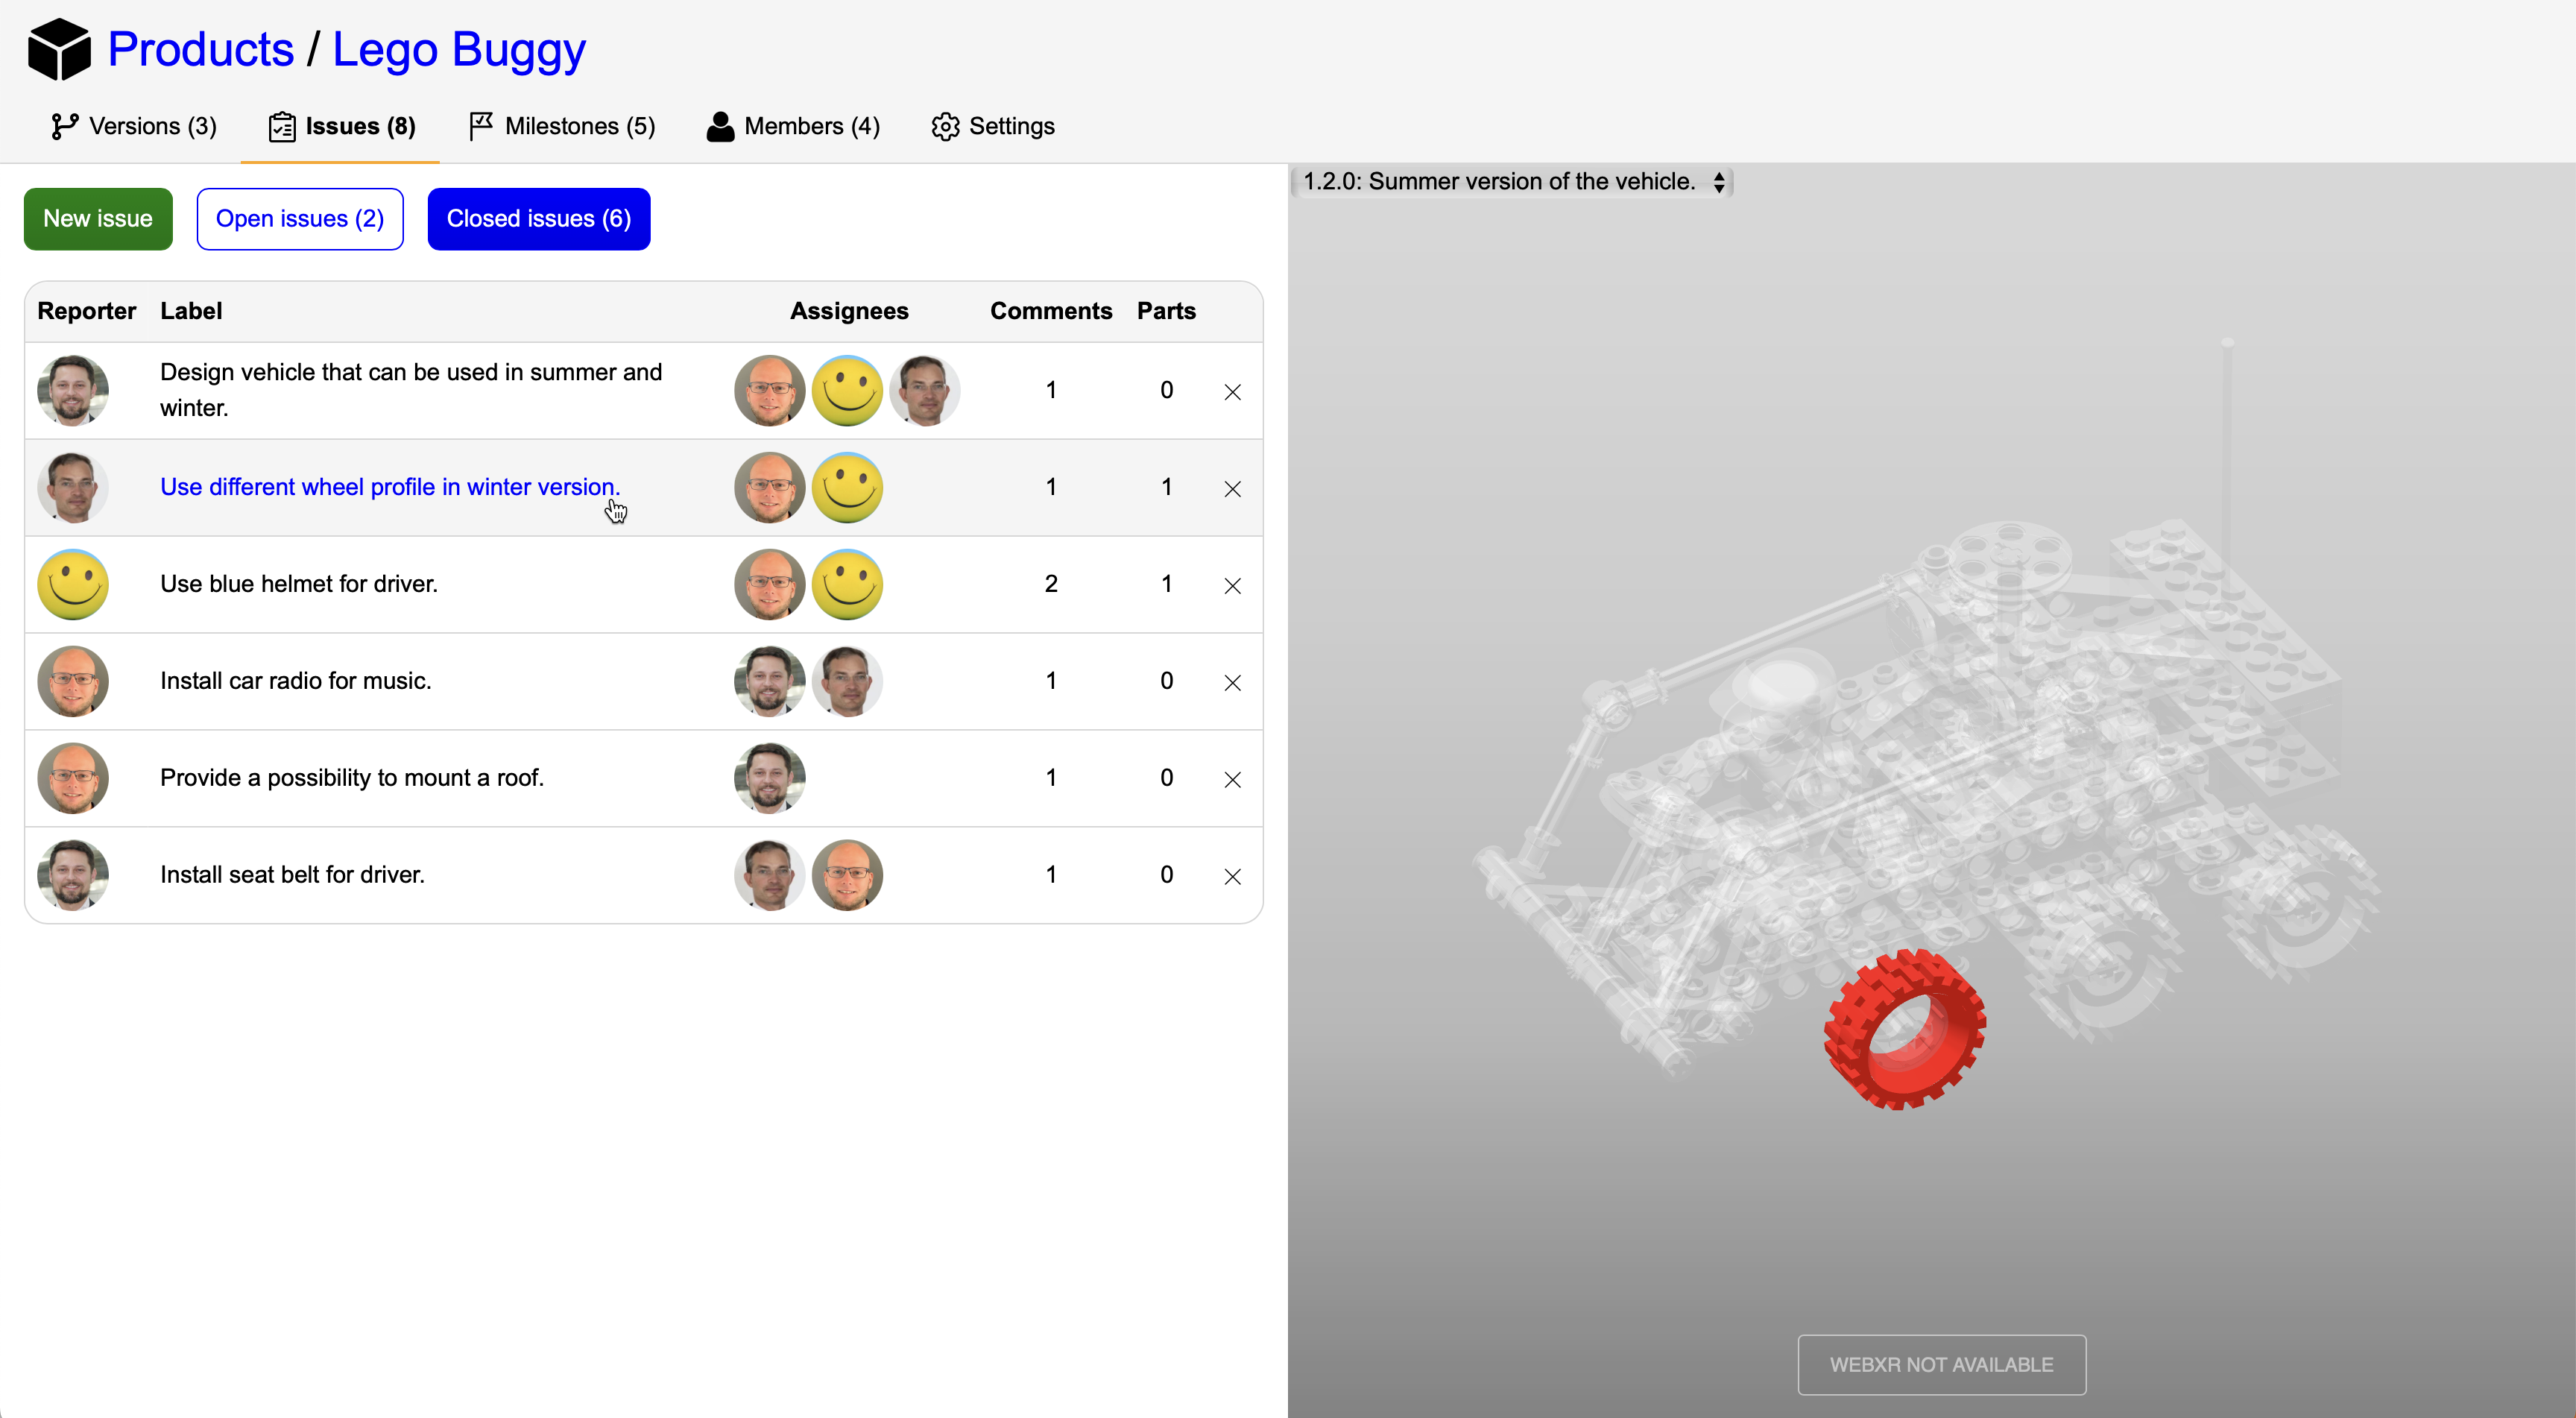
\includegraphics[width=\columnwidth]{issueviewselectedpart.png}
        \caption{Issue view}
        \label{fig: issueview}
    \end{figure}

    \subsubsection*{ProductIssueSettings view}
    The ProductIssueSettings view allows to create new issues for the product [see Fig. \ref{fig: issuesettingsview} on page~\pageref{fig: issuesettingsview}]. The label, the text, the milestone and the assignees can be defined. An existing milestone can be selected with the dropdown menu. An issue must not be assigned to a milestone. This choice lies by the user. 
    As in the ProductIssue view, the model of the desired version can also be selected here via dropdown menu on the 3D view.
    The \textit{text} field in the ProductIssueSettings view represents the first comment in an issue. By clicking on the part, the part gets included in the comment as markdown text. If a comment includes a marked part when created, the marking of the respective part is saved to the associated product version.
    The Save button closes the settings, and you return to the ProductIssue view where the new issue is visible.

    \begin{figure}[h]
        \centering
        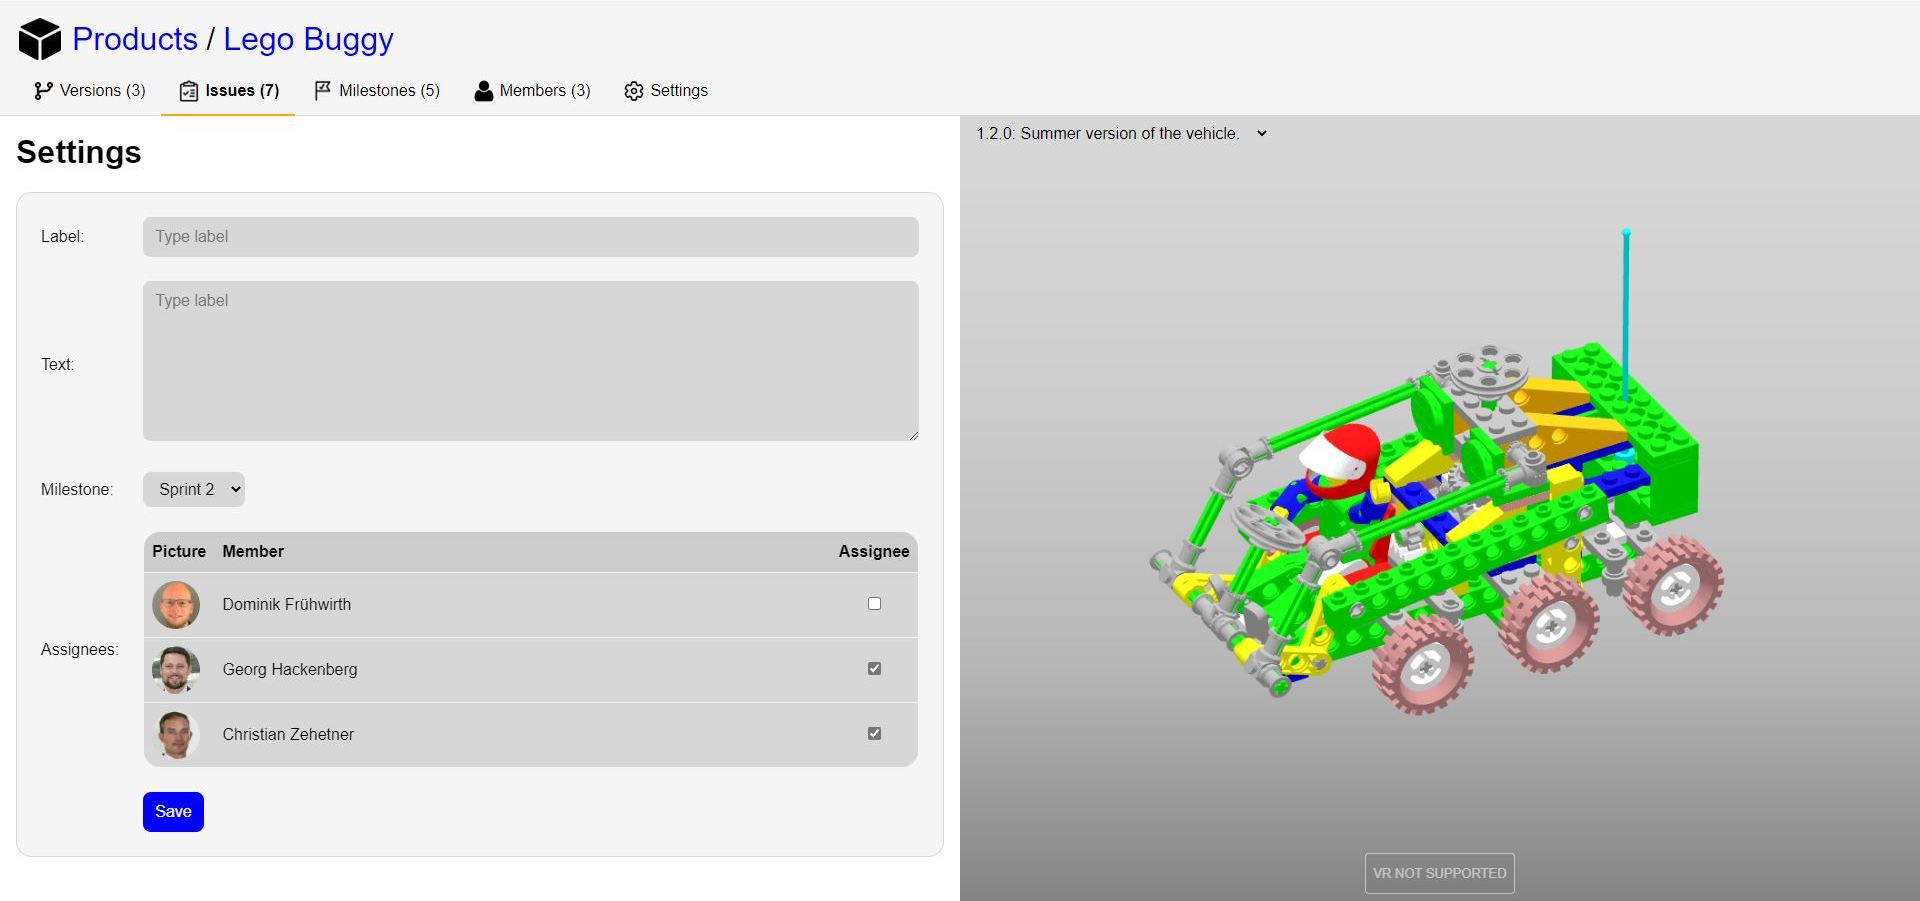
\includegraphics[width=\columnwidth]{issuesettingsview.JPG}
        \caption{Issuesettings view}
        \label{fig: issuesettingsview}
    \end{figure}

    \subsubsection*{ProductIssueComment view}
    Clicking on an issue in the Issue view opens the corresponding ProductIssueComment view.  Here you have the possibility to discuss the issue. 
    For this purpose, in the new comment box a text can be entered. This text field supports markdown.
    Like in the ProductIssueSettings view you can click on a part of the 3D model to mark a part as markdown[see Fig. \ref{fig: commentselectedpartview} on page~\pageref{fig: commentselectedpartview}]. In the course of a discussion, several parts can be marked in this way.
    A comment can also be used to close an issue by clicking the close button. This issue will then be found in Closed Issues in the ProductIssue view. With the comment function it is also possible to reopen the issue in the same way. The Close button displays the text Reopen when an issue is closed. In the upper right corner of the ProductIssueComment view there is a button to edit the selected issue. For example, the issue can be assigned to another Milestone or other attributes like the label, text or the list of assignees can be changed [see Fig. \ref{fig: issuesettingsview} on page~\pageref{fig: issuesettingsview}].

    \begin{figure}[h]
        \centering
        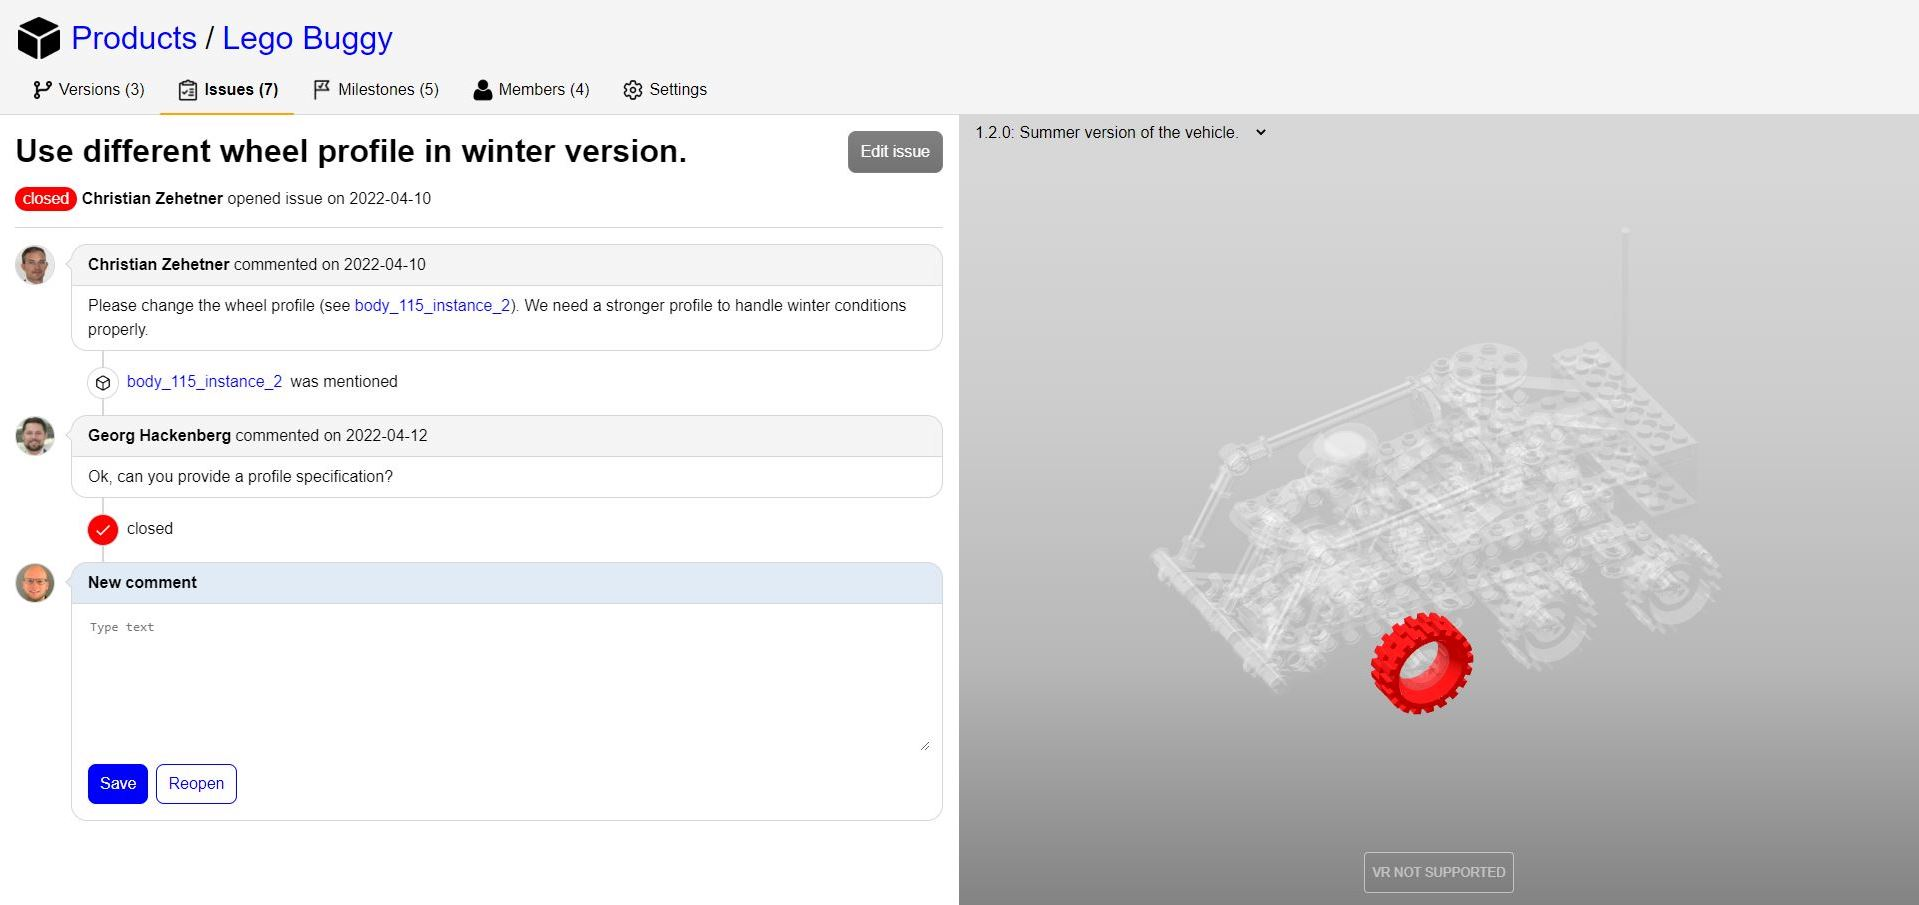
\includegraphics[width=\columnwidth]{commentselectedpartview.JPG}
        \caption{Selected part in ProductIssueComment view}
        \label{fig: commentselectedpartview}
    \end{figure}

    \subsubsection*{ProductMilestone view}
    The ProductMilestone view can be accessed via the Milestones link [see Fig. \ref{fig: milestoneview} on page~\pageref{fig: milestoneview}]. A table shows who created the milestone, its name, start date, end date and the progress. For each milestone two progress bars are displayed. The first one shows the date progress of a milestone by calculating \textit{100 * (nowDate - startDate) / (endDate - startDate)}. The second bar shows the issue progress of a milestone by calculating \textit{100 * number of closedIssues / number of allIssues}.
    A click on the New Milestone button leads to the ProductMilestoneSettings view. Here the attributes of a milestone can be adjusted and saved. The new or edited Milestone than show up in the ProductMilestone view.

    \begin{figure}[h]
        \centering
        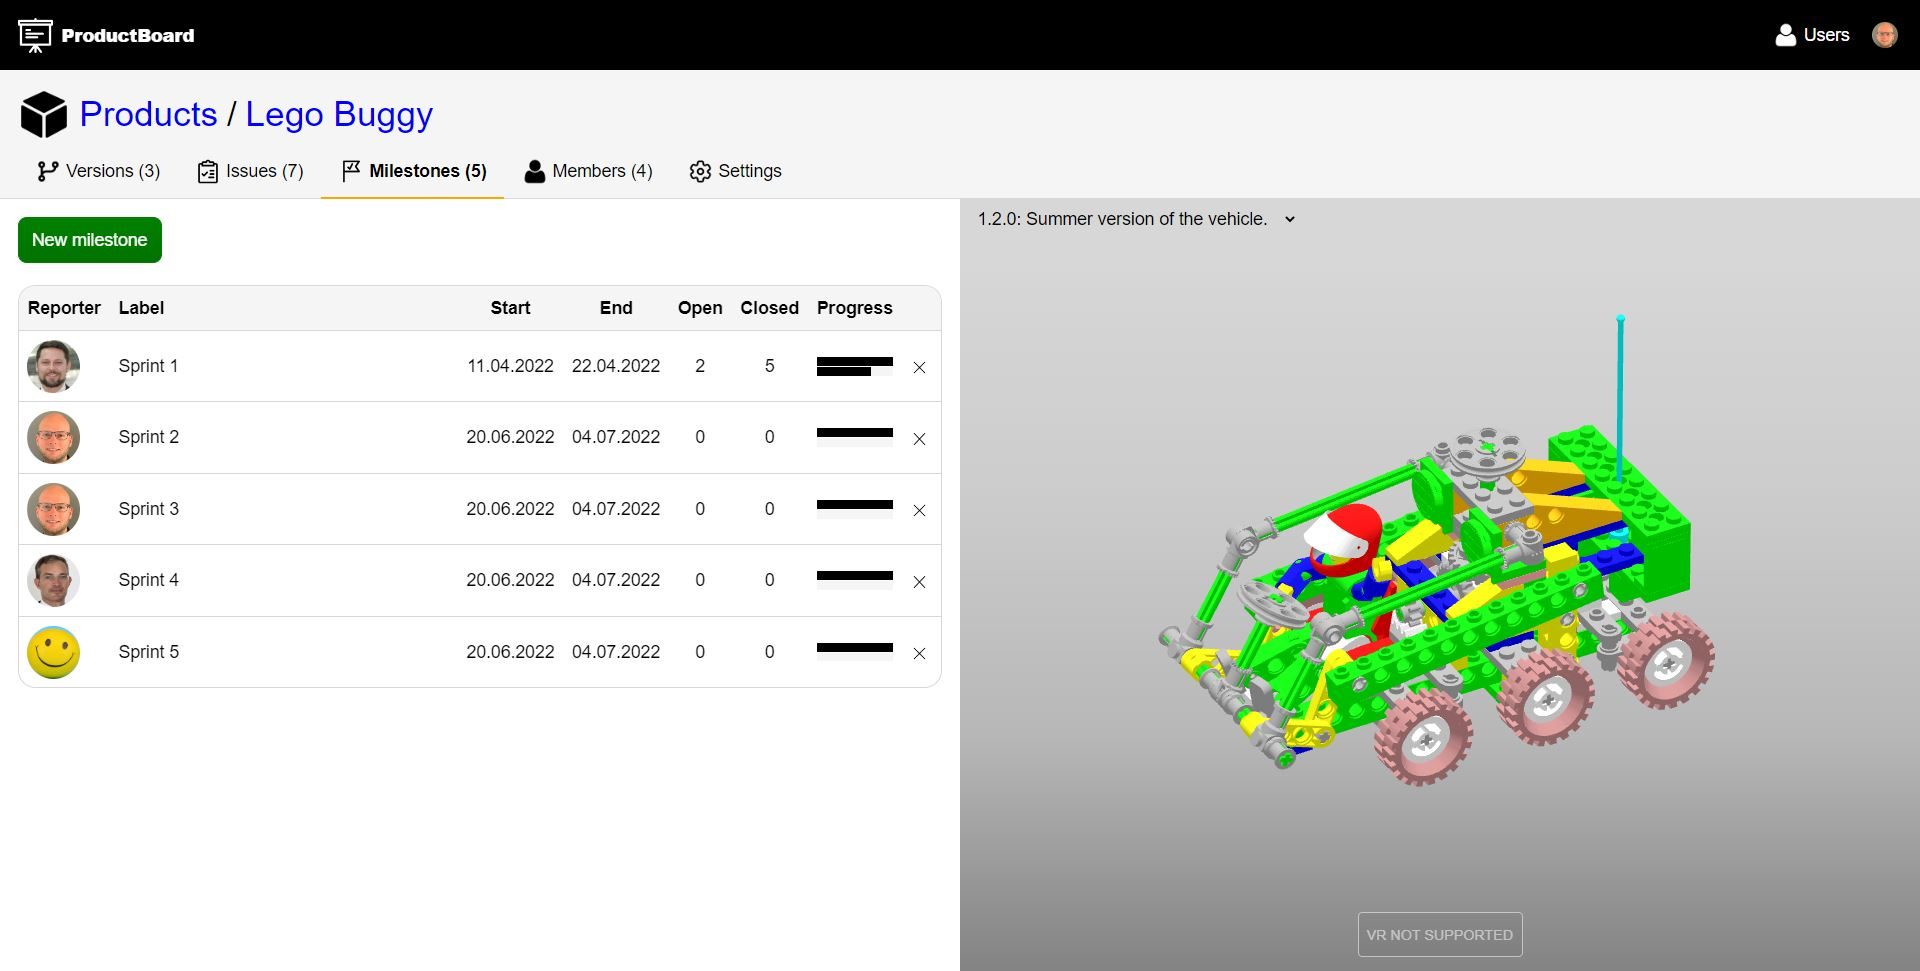
\includegraphics[width=\columnwidth]{milestoneview.JPG}
        \caption{ProductMilestone view}
        \label{fig: milestoneview}
    \end{figure}

    \subsubsection*{ProductMilestoneIssue view}
    If a milestone is selected, a table with the attached issues is displayed [see Fig. \ref{fig: sprintview} on page~\pageref{fig: sprintview}]. This table is identical to the one in the ProductIssue view. Here you can also filter by open and closed issues. On the right side a burn down chart is displayed which shows the current progress of the milestone. The chart shows the start date, the end date, the number of issues and the progress until the current day. In the chart, the green line represents the target burndown and the blue graph the actual burndown. The target burndown distributes the open issues over the time span. The actual burndown drops by one for each issue that is closed.  Like in the ProductMilestone view, a click Edit Milestone button leads to the ProductMilestoneSettings view where the attributes of a milestone can be changed.

    \begin{figure}[h]
        \centering
        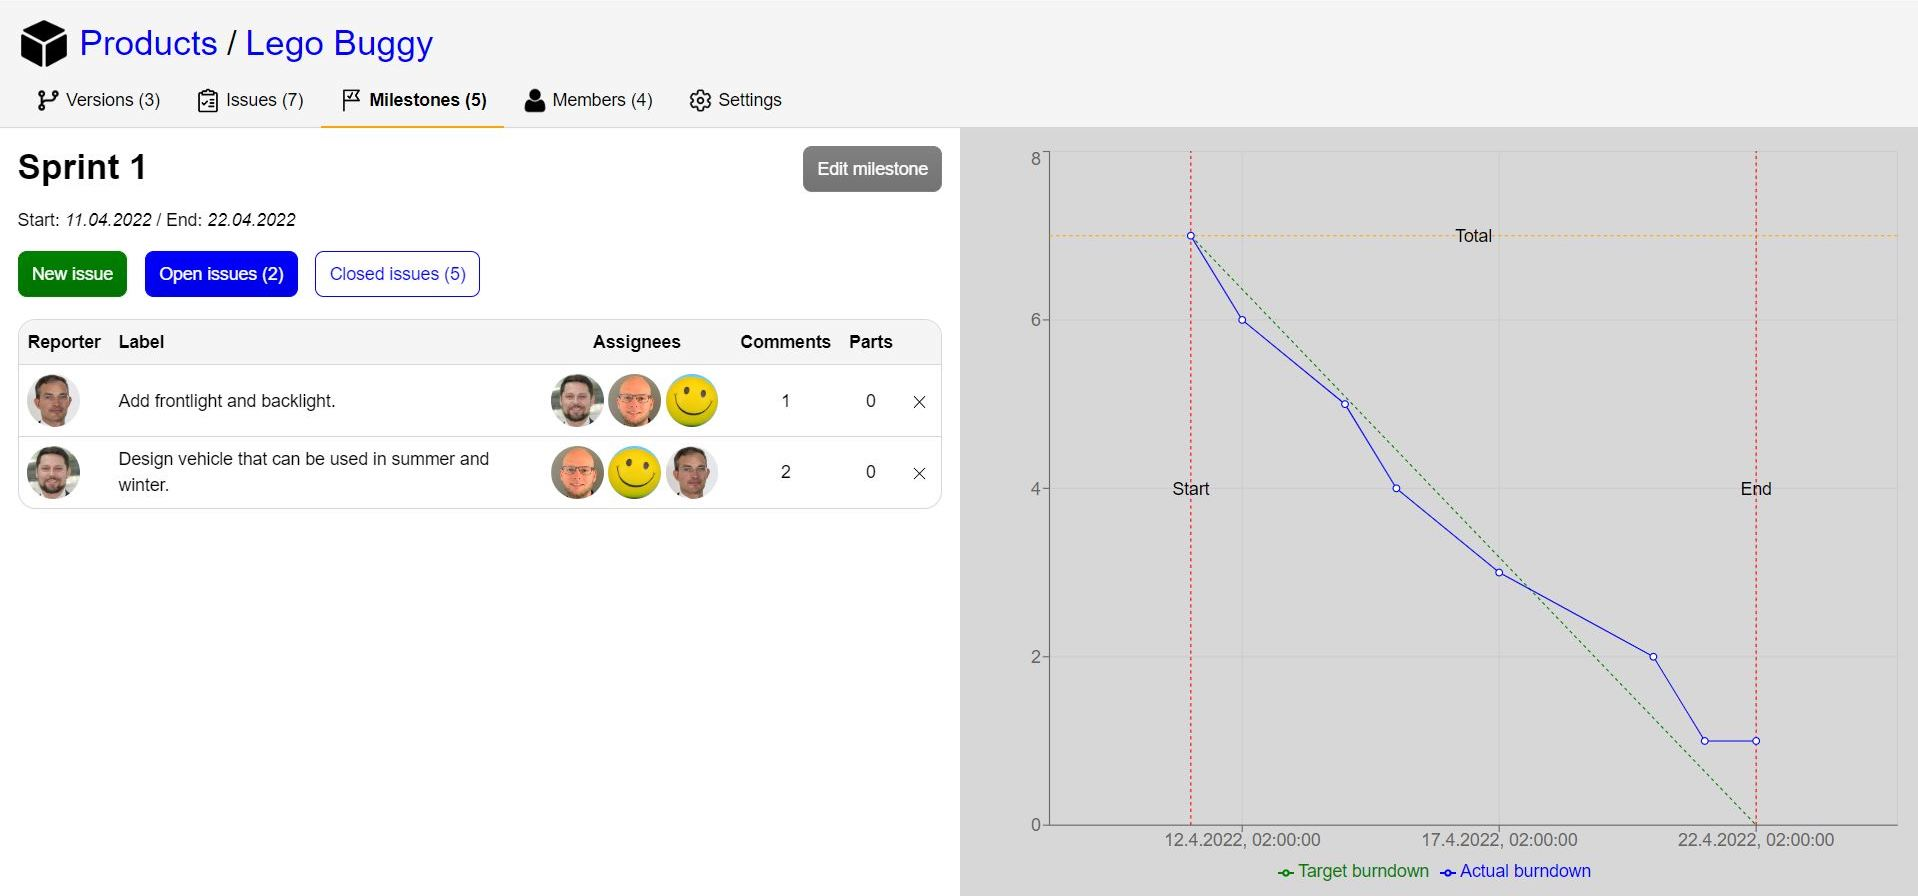
\includegraphics[width=\columnwidth]{sprintview.JPG}
        \caption{ProductMilestoneIssue view}
        \label{fig: sprintview}
    \end{figure}

    \subsubsection*{ProductMember view}
    To distribute the rights for a product, members are added to an existing product via the user interface. In the ProductMember view, a table shows all members who have access to the selected product [see Fig. \ref{fig: memberview} on page~\pageref{fig: memberview}]. The table shows the user picture and the name of the user. The role column defines which rights the respective member has. At the moment there are three roles: \textit{manager, engineer, customer} as explained in the permission model.. As with every overview table, objects can be deleted from the list by clicking on the X button. The button New Member leads to the ProductMemberSettings view where new members can be added.
    
    \begin{figure}[h]
        \centering
        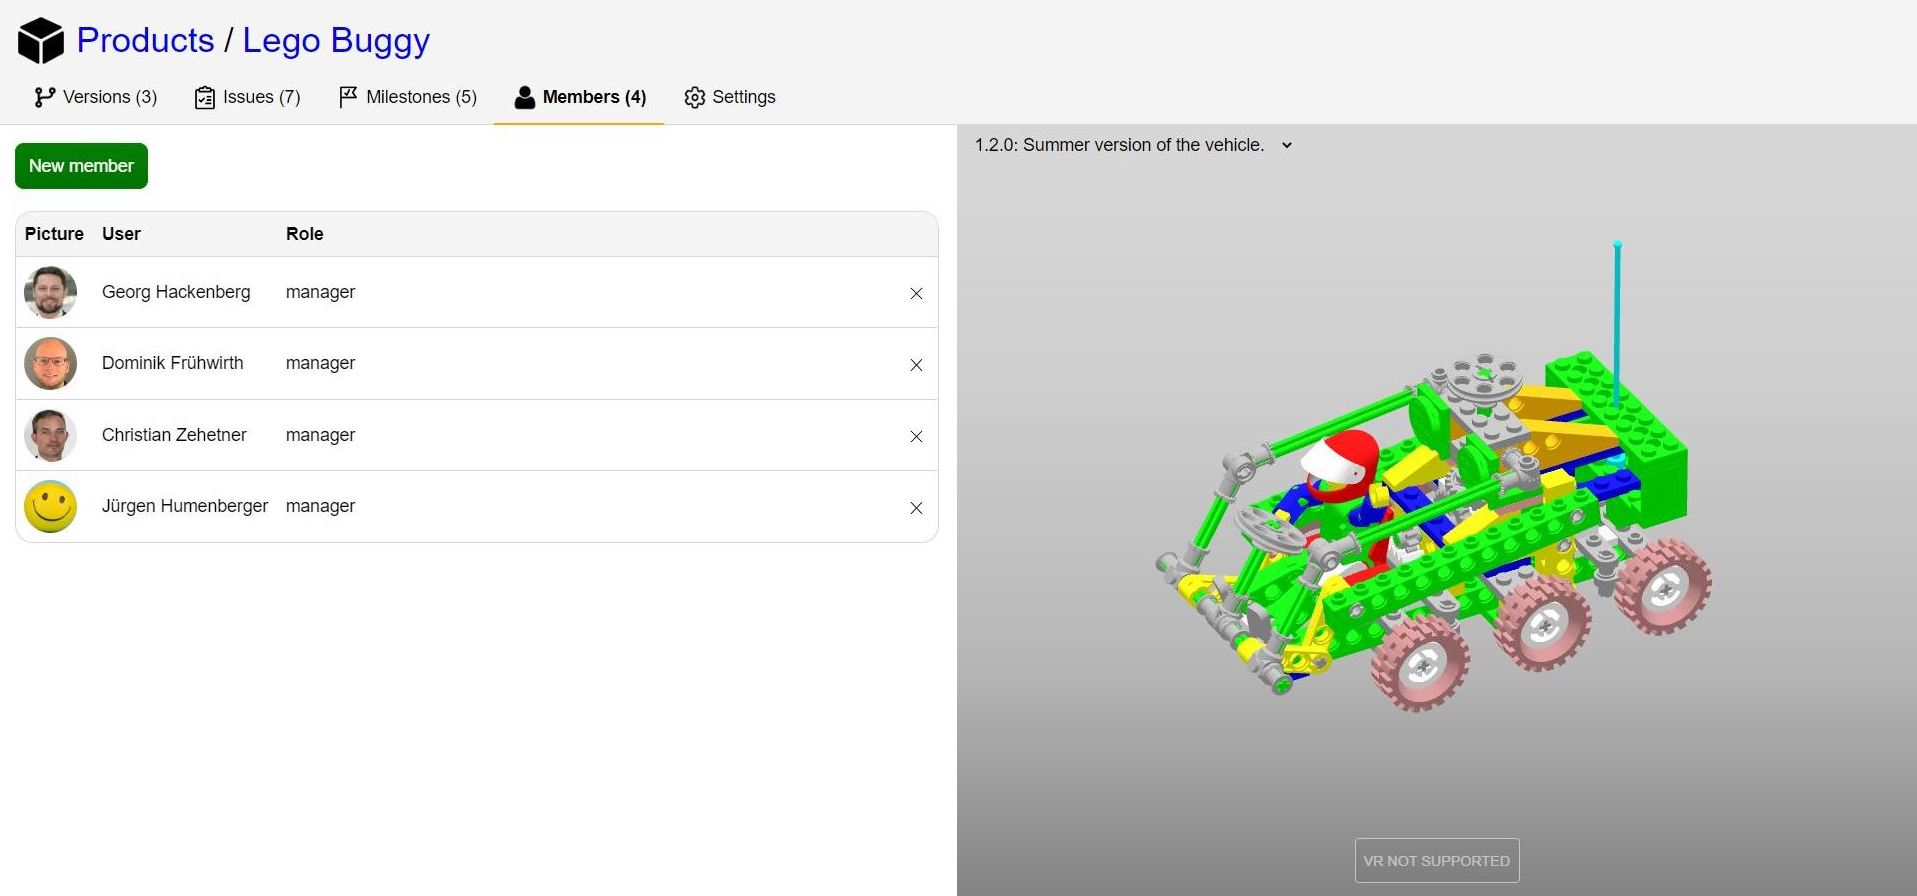
\includegraphics[width=\columnwidth]{memberview.JPG}
        \caption{Member view}
        \label{fig: memberview}
    \end{figure}
